\documentclass[aspectratio=169,11pt]{beamer}

% Packages
\usepackage[utf8]{inputenc}
\usepackage[T1]{fontenc}
\usepackage{lmodern}
\usepackage{microtype}
\usepackage{amsmath,amssymb}
\usepackage{booktabs}
\usepackage{graphicx}
\usepackage{tikz}
\usepackage{pgfplots}
\usepackage{xcolor}
\usepackage{ragged2e}
\usepackage{colortbl}
\usepackage{array}
\usepackage{hyperref}
\usepackage{adjustbox}

\usetikzlibrary{shapes.geometric, arrows.meta, positioning, calc, backgrounds, decorations.pathreplacing, shadows, fadings}
\pgfplotsset{compat=1.18}

% --- Color Palette: Warm Professional ---
\definecolor{DeepNavy}{HTML}{2E4057}
\definecolor{Teal}{HTML}{048A81}
\definecolor{WarmOrange}{HTML}{E85D04}
\definecolor{SoftPurple}{HTML}{9D4EDD}
\definecolor{WarmGray}{HTML}{6C757D}
\definecolor{LightGray}{HTML}{E9ECEF}
\definecolor{Cream}{HTML}{FBF8F1}
\definecolor{DeepRed}{HTML}{D62828}
\definecolor{Gold}{HTML}{D4A03A}
\definecolor{SoftWhite}{HTML}{FAFAFA}

% Beamer colors
\setbeamercolor{normal text}{fg=DeepNavy, bg=SoftWhite}
\setbeamercolor{structure}{fg=DeepNavy}
\setbeamercolor{alerted text}{fg=DeepRed}
\setbeamercolor{example text}{fg=Teal}
\setbeamercolor{frametitle}{fg=DeepNavy, bg=SoftWhite}
\setbeamercolor{title}{fg=DeepNavy}
\setbeamercolor{subtitle}{fg=WarmGray}
\setbeamercolor{block title}{bg=DeepNavy, fg=SoftWhite}
\setbeamercolor{block body}{bg=LightGray, fg=DeepNavy}
\setbeamercolor{itemize item}{fg=WarmOrange}
\setbeamercolor{itemize subitem}{fg=Gold}

% Fonts
\usefonttheme{professionalfonts}
\setbeamerfont{title}{size=\huge, series=\bfseries}
\setbeamerfont{frametitle}{size=\Large, series=\bfseries}

% Strip chrome
\setbeamertemplate{navigation symbols}{}
\setbeamertemplate{headline}{}

% Minimal footline
\setbeamertemplate{footline}{%
    \hfill
    \begin{beamercolorbox}[wd=3cm,ht=2.5ex,dp=1ex,right,rightskip=0.6cm]{page number}
        \usebeamercolor[fg]{WarmGray}\scriptsize\insertframenumber
    \end{beamercolorbox}
    \vspace{0.3cm}
}

% Bullets
\setbeamertemplate{itemize item}{\footnotesize\raisebox{0.3ex}{\tikz\fill[WarmOrange] (0,0) circle (0.45ex);}}
\setbeamertemplate{itemize subitem}{\footnotesize\raisebox{0.3ex}{\tikz\fill[Gold] (0,0) circle (0.35ex);}}

% Custom commands
\newcommand{\transitionslide}[2]{%
    {\setbeamercolor{normal text}{fg=SoftWhite,bg=DeepNavy}
    \begin{frame}[plain]\vfill\begin{center}
        {\huge\bfseries\textcolor{Gold}{#1}}\\[0.6cm]
        {\large\textcolor{LightGray}{#2}}
    \end{center}\vfill\end{frame}}
}

\begin{document}

\begin{frame}
\title{Granular Instrumental Variables}
\subtitle{Estimating Aggregate Effects of Firm Shocks on Wages}
\author{Macro Lab Group Presentation}
\date{}
\titlepage
\end{frame}

\begin{frame}
\frametitle{Do shocks to superstar firms drive aggregate wage dynamics?}

\begin{columns}
\begin{column}{0.6\textwidth}
\vspace{0.5cm}
{\Large
When a dominant employer experiences an unexpected surge in productivity, local and aggregate wages often respond.
}

\vspace{0.8cm}
{\Large
But how much of that response is causal, and how much is driven by common macroeconomic trends?
}
\end{column}
\begin{column}{0.4\textwidth}
\begin{center}
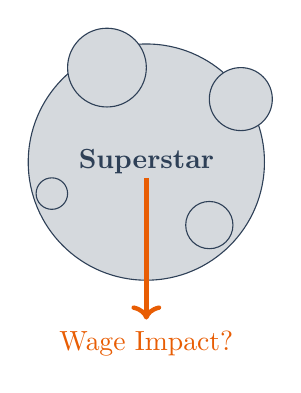
\begin{tikzpicture}
    % Representing concentration
    \foreach \x/\y/\s in {0/0/1.5, 1.2/0.8/0.4, 0.8/-0.8/0.3, -0.5/1.2/0.5, -1.2/-0.4/0.2} {
        \draw[fill=DeepNavy!20, draw=DeepNavy] (\x,\y) circle (\s);
    }
    \node[text=DeepNavy, font=\bfseries] at (0,0) {Superstar};
    \draw[->, ultra thick, WarmOrange] (0, -0.2) -- (0, -2) node[below] {Wage Impact?};
\end{tikzpicture}
\end{center}
\end{column}
\end{columns}

\end{frame}

\begin{frame}
\frametitle{Endogenous aggregate shocks confound the effect of large firms}

\vspace{0.5cm}
\begin{columns}
\begin{column}{0.5\textwidth}
{\Large
We want to estimate the elasticity of wages to labor demand.
}

\vspace{0.5cm}
{\Large
The fundamental challenge:
}
\end{column}
\begin{column}{0.5\textwidth}
\begin{center}
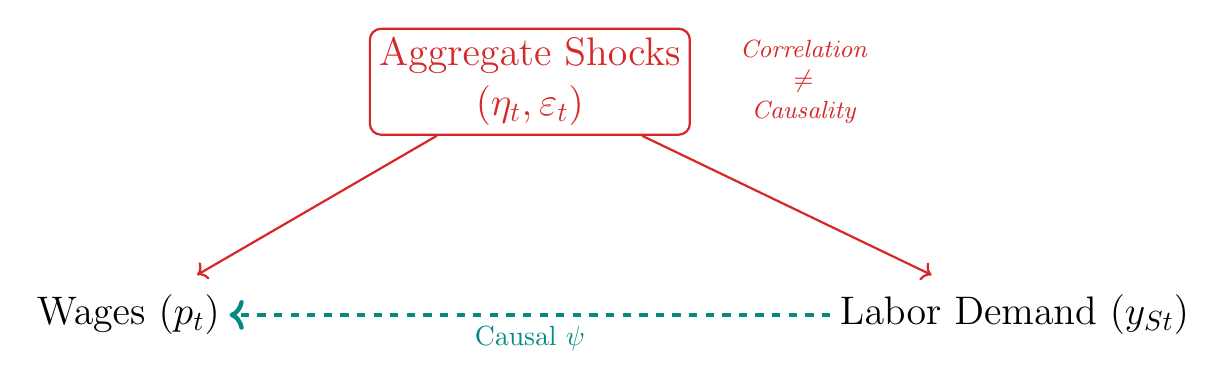
\begin{tikzpicture}[node distance=2.5cm, align=center]
  \node (common) [draw, DeepRed, thick, rounded corners, font=\Large, text=DeepRed, minimum width=3cm, minimum height=1cm] {Aggregate Shocks\\($\eta_t, \varepsilon_t$)};
  \node (wages) [below left=of common, font=\Large, minimum width=2cm, minimum height=1cm] {Wages ($p_t$)};
  \node (demand) [below right=of common, font=\Large, minimum width=3cm, minimum height=1cm] {Labor Demand ($y_{St}$)};
  
  \draw[->, thick, DeepRed] (common) -- (wages);
  \draw[->, thick, DeepRed] (common) -- (demand);
  \draw[->, ultra thick, dashed, Teal] (demand) -- (wages) node[midway, below] {Causal $\psi$};
  
  \node[right=0.5cm of common, text=DeepRed, font=\small\itshape] {Correlation\\$\neq$\\Causality};
\end{tikzpicture}
\end{center}
\end{column}
\end{columns}

\end{frame}

\transitionslide{A Simple Model}{Section III.A of Gabaix and Koijen (2022)}

\begin{frame}
\frametitle{A simple model of aggregate and idiosyncratic shocks}

\begin{columns}
\begin{column}{0.5\textwidth}
The system is given by:

\vspace{0.5cm}
\begin{align}
p_t &= \psi y_{St} + \varepsilon_t \tag{38} \\[0.5cm]
y_{it} &= \phi^d p_t + \eta_t + u_{it} \tag{39}
\end{align}

\vspace{0.5cm}
{\small Where $y_{St} = \sum_i S_i y_{it}$ is the size-weighted aggregate outcome.}
\end{column}
\begin{column}{0.5\textwidth}
\begin{center}
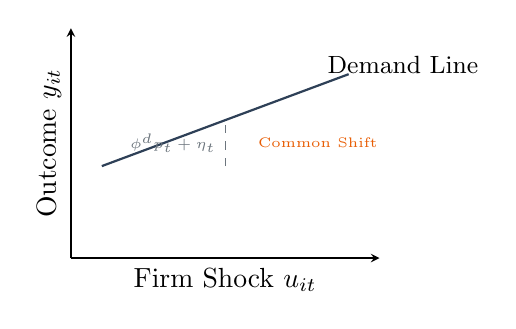
\begin{tikzpicture}
    \begin{axis}[
        width=5.5cm, height=4.5cm,
        axis lines=left,
        xlabel={Firm Shock $u_{it}$},
        ylabel={Outcome $y_{it}$},
        ticks=none,
        domain=-2:2,
        samples=10,
        xmin=-2.5, xmax=2.5,
        ymin=-2, ymax=3,
        clip=false
    ]
        \addplot[DeepNavy, thick] {0.5*x + 1}; % Common level + idiosyncratic
        \node[right, font=\small] at (axis cs: 1.5, 2.2) {Demand Line};
        \draw[dashed, WarmGray] (axis cs: 0, 0) -- (axis cs: 0, 1) node[midway, left, font=\tiny] {$\phi^d p_t + \eta_t$};
        \node[WarmOrange, font=\tiny] at (axis cs: 1.5, 0.5) {Common Shift};
    \end{axis}
\end{tikzpicture}
\end{center}
\end{column}
\end{columns}

\end{frame}

\begin{frame}
\frametitle{Constructing the Granular Instrumental Variable ($z_t$)}

\vspace{0.5cm}
{\Large
The GIV exploits the difference between size-weighted and equal-weighted averages.
}

\vspace{1cm}
\begin{center}
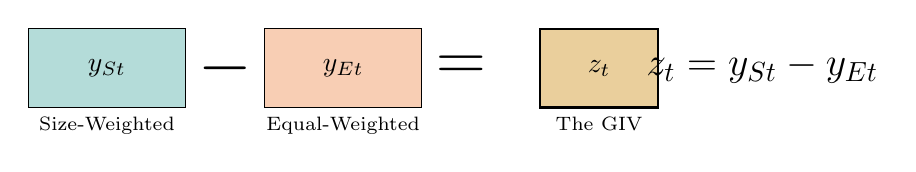
\begin{tikzpicture}
    % Size-weighted representation
    \begin{scope}[shift={(0,0)}]
        \draw[fill=Teal!30] (0,0) rectangle (2,1);
        \node at (1,0.5) {$y_{St}$};
        \node[below] at (1,0) {\scriptsize Size-Weighted};
    \end{scope}
    
    \node at (2.5, 0.5) {\Huge $-$};
    
    % Equal-weighted representation
    \begin{scope}[shift={(3,0)}]
        \draw[fill=WarmOrange!30] (0,0) rectangle (2,1);
        \node at (1,0.5) {$y_{Et}$};
        \node[below] at (1,0) {\scriptsize Equal-Weighted};
    \end{scope}
    
    \node at (5.5, 0.5) {\Huge $=$};
    
    % GIV representation
    \begin{scope}[shift={(6.5,0)}]
        \draw[fill=Gold!50, thick] (0,0) rectangle (1.5,1) node[midway] (GoldNode) {$z_t$};
        \node[below] at (0.75,0) {\scriptsize The GIV};
    \end{scope}
    
    \node[right=0.2cm of GoldNode] {\Large $z_t = y_{St} - y_{Et}$};
\end{tikzpicture}
\end{center}

\end{frame}

\begin{frame}
\frametitle{The GIV isolates purely idiosyncratic firm shocks}

\vspace{0.5cm}
\begin{center}
\begin{adjustbox}{max width=\textwidth}
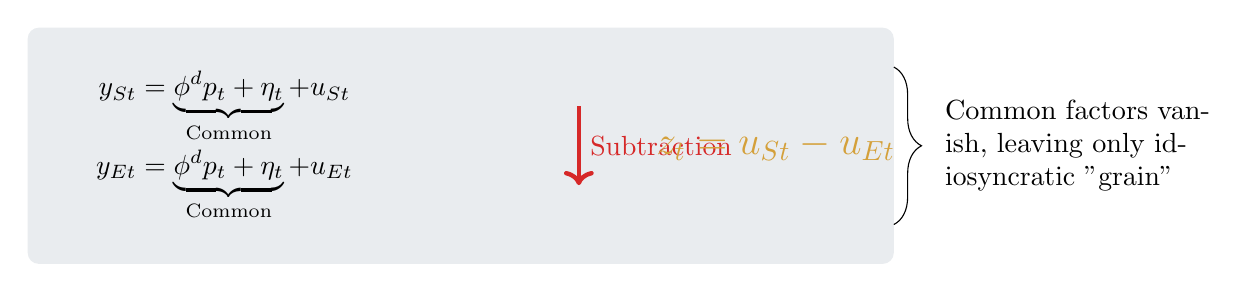
\begin{tikzpicture}[node distance=1cm]
    \node (syst) [fill=LightGray, minimum width=11cm, minimum height=3cm, rounded corners] {};
    
    \node (st) at (-3, 0.5) {$y_{St} = \underbrace{\phi^d p_t + \eta_t}_{\text{Common}} + u_{St}$};
    \node (et) at (-3, -0.5) {$y_{Et} = \underbrace{\phi^d p_t + \eta_t}_{\text{Common}} + u_{Et}$};
    
    \draw[->, ultra thick, DeepRed] (1.5, 0.5) -- (1.5, -0.5) node[midway, right] {Subtraction};
    
    \node[Gold, font=\Large\bfseries] at (4, 0) {$z_t = u_{St} - u_{Et}$};
    
    \draw[decorate, decoration={brace, amplitude=10pt}] (5.5, 1) -- (5.5, -1) node[midway, right=15pt, text width=3.5cm] {Common factors vanish, leaving only idiosyncratic "grain"};
\end{tikzpicture}
\end{adjustbox}
\end{center}

\end{frame}

\begin{frame}
\frametitle{GIV precision relies on concentrated labor markets}

\begin{columns}
\begin{column}{0.5\textwidth}
{\Large
For the instrument to be strong, we need:
}
\vspace{0.5cm}
\begin{enumerate}
    \item \textbf{A Large Excess Herfindahl ($h$):} Concentrated markets.
    \item \textbf{Volatile Micro-Shocks ($\sigma_u$)}
\end{enumerate}
\end{column}
\begin{column}{0.5\textwidth}
\begin{center}
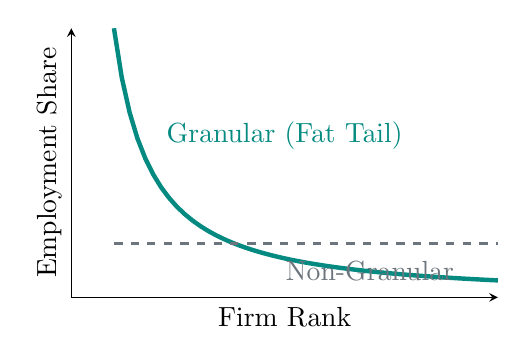
\begin{tikzpicture}
    \begin{axis}[
        width=7cm, height=5cm,
        axis lines=left,
        xlabel={Firm Rank},
        ylabel={Employment Share},
        xmin=0, xmax=10,
        ymin=0, ymax=1,
        ticks=none
    ]
        \addplot[Teal, ultra thick, domain=1:10, samples=50] {1/x^1.2};
        \node[Teal] at (axis cs: 5, 0.6) {Granular (Fat Tail)};
        
        \addplot[WarmGray, thick, dashed, domain=1:10, samples=50] {0.2};
        \node[WarmGray] at (axis cs: 7, 0.1) {Non-Granular};
    \end{axis}
\end{tikzpicture}
\end{center}
\end{column}
\end{columns}

\end{frame}

\begin{frame}
\frametitle{The GIV yields both supply and demand elasticities}

\vspace{0.5cm}
\begin{columns}
\begin{column}{0.45\textwidth}
\begin{block}{Supply Side}
\centering
$\psi = \frac{\mathbb{E}[p_t z_t]}{\mathbb{E}[y_{St} z_t]}$
\end{block}
\end{column}
\begin{column}{0.1\textwidth}
\centering \Huge \&
\end{column}
\begin{column}{0.45\textwidth}
\begin{block}{Demand Side}
\centering
$\phi^d = \frac{\mathbb{E}[y_{Et} z_t]}{\mathbb{E}[p_t z_t]}$
\end{block}
\end{column}
\end{columns}

\vspace{0.8cm}
\begin{center}
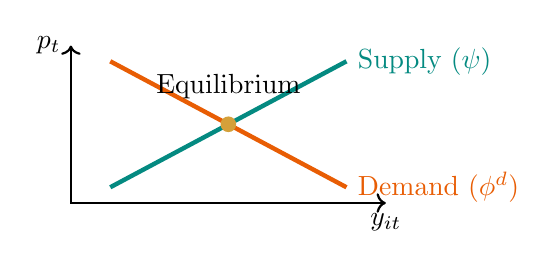
\begin{tikzpicture}
    \draw[thick, <->] (0,2) node[left]{$p_t$} -- (0,0) -- (4,0) node[below]{$y_{it}$};
    \draw[Teal, ultra thick] (0.5, 0.2) -- (3.5, 1.8) node[right]{Supply ($\psi$)};
    \draw[WarmOrange, ultra thick] (0.5, 1.8) -- (3.5, 0.2) node[right]{Demand ($\phi^d$)};
    \node[Gold, circle, fill, inner sep=2pt] at (2,1) {};
    \node[above=0.2cm] at (2,1) {Equilibrium};
\end{tikzpicture}
\end{center}

\end{frame}

\end{document}
